%----------------------------------------------------------------------------------------
%	PACKAGES AND THEMES
%----------------------------------------------------------------------------------------

\documentclass{beamer}

\mode<presentation> {

\usetheme{Singapore}
\usecolortheme{seahorse}

 % To remove the footer line in all slides uncomment this line
\setbeamertemplate{footline}{}

%\setbeamertemplate{footline}[page number] % To replace the footer line in all slides with a simple slide count uncomment this line
%\setbeamertemplate{navigation symbols}{} % To remove the navigation symbols from the bottom of all slides uncomment this line
}
\usepackage[export]{adjustbox}
\usepackage{amsmath}
\usepackage{graphicx} % Allows including images
\usepackage{booktabs} % Allows the use of \toprule, \midrule and \bottomrule in tables
\usepackage[comma]{natbib}

% CAPTIONS
\usepackage{subfig}

%\usepackage{sectsty} % Allows customizing section commands
%\allsectionsfont{\centering \normalfont\scshape} % Make all sections centered, the default font and small caps

\newcommand{\mb}{\mathbf}
\newcommand{\tb}{\textbf}
\newcommand{\ti}{\textit}
\newcommand{\ul}{\underline}
\newcommand{\bi}{\begin{itemize}}
\newcommand{\ei}{\end{itemize}}
\newcommand{\be}{\begin{enumerate}}
\newcommand{\ee}{\end{enumerate}}

% Non-shown text to appear gray
\setbeamercovered{transparent}

% NO HYPHENATION TEST
\usepackage[none]{hyphenat}

% FANCY FOOTNOTE SYMBOLS
\renewcommand*{\thefootnote}{\fnsymbol{footnote}}

\renewcommand{\baselinestretch}{1.2}

% LOGO
\logo{
	\centering
	
\includegraphics[scale=0.2]{epic_logo}
}

%%%%%%%%%%%%%%%%%%%%%%%%%%%%%%%%%%%%%%%%%%%%%%%%

\title[Server]{The Data Project}
\institute{\large{EPIC RA Orientation}}
\date{August 20, 2018}

%%%%%%%%%%%%%%%%%%%%%%%%%%%%%%%%%%%%%%%%%%%%%%%%%%%%%%%%%%%%%%%%%%%%%
\begin{document}

\begin{frame}
	\titlepage
\end{frame}

\section{Motivation}
\begin{frame}
\frametitle{Why are we doing (another) data task?}
There is a lot of stuff we wish we knew when we were in your shoes.
\\[1em]\pause
At times, all of the new things you learn can be overwhelming.
\\[1em]\pause
To make the transition a little easier, we would like to teach you a few of the vital things an Epic RA needs.
\\[1em]\pause
``Learning by doing" $\implies$ data project!
\end{frame}

\begin{frame}
\frametitle{What will I be learning?}
From this project, we hope to introduce you to the following languages, packages, and software:
\be
\item Stata (not STATA)
\item R
\item RSpatial/ArcGIS
\item Python
\item \LaTeX/Lyx
\item Bash 
\item Git/Github
\ee

Beyond that, we would like to teach you some econometric methods along the way.
\end{frame}

\section{Project Background}
\begin{frame}
\frametitle{Superfund}
\small{In the late 1970s, toxic waste dumps such as Love Canal and Valley of the Drums received national attention when the public learned about the risks to human health and the environment posed by contaminated sites.
\\[1em]\pause
In response, Congress established the Comprehensive Environmental Response, Compensation and Liability Act (CERCLA) in 1980.
\\[1em]\pause
CERCLA is informally called Superfund. It allows EPA to clean up contaminated sites. It also forces the parties responsible for the contamination to either perform cleanups or reimburse the government for EPA-led cleanup work [\cite{epa}].} 
\end{frame}

\begin{frame}
\frametitle{Superfund (cont.)}
For a site to be considered for cleanup, the EPA must place the site on the National Priorities List (NPL). 
\\[1em]\pause
To be placed on the NPL, the EPA undergoes a series of investigations on the site to determine the risk it poses to human health.
\\[1em]\pause
Cleaning a site can be a long an arduous task. Some sites take over 20 years to clean completely. 
\end{frame}

\begin{frame}
\frametitle{Gary, Indiana}
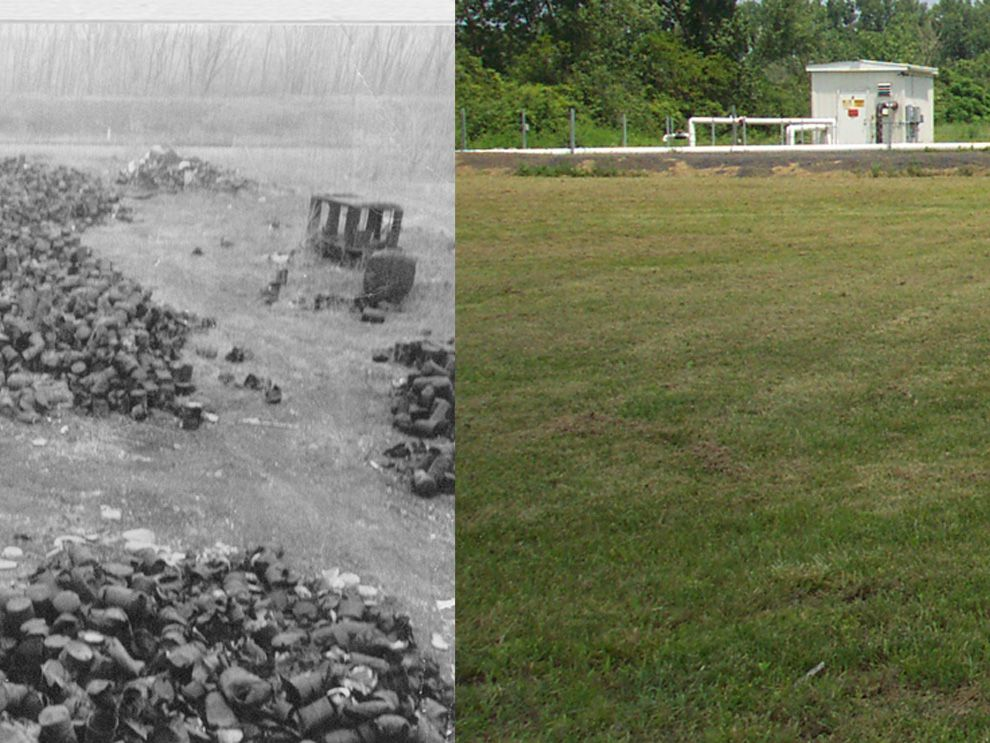
\includegraphics[width=3in, center]{superfund}
\scriptsize{ A fire destroyed between 50,000 and 60,000 barrels of toxic materials at a dump in Gary, Indiana, in 1977. It became a Superfund site in 1986, and cleanup ended in 2009 [\cite{natgeo}].}

\tiny{ Photograph by Mick Haas, EPA 1978, and photograph (right) by Mary Schons, 2009}
\end{frame}

\section{Your Task}
\begin{frame}
\frametitle{Does the public value the Superfund cleanups?}
Are we able to quantify to local welfare benefits of the Superfund cleanup to former hazardous waste sites?
\\[1em]\pause
One way we can measure this is by comparing housing prices before and after a cleanup. A researcher could potentially do that with the following regression
\[ HP_{i,t_1} = \alpha + \beta NPL_{i,t_1} +\textbf{X}_{i,t_0}' \gamma  + \varepsilon_{i,t_1} \]
\\[1em]\pause
Here, $HP$ represents housing prices, $NPL$ is a dummy for NPL status, and \textbf{X} is a vector of controls. All data is recorded at the site level $i$ both in the pre-treatment period ($t_0$) and the post-treatment period ($t_1$).
\end{frame}

\begin{frame}
\frametitle{Why would this framework answer our question correctly?}
HENRY HERE PLACE YOUR HEDONIC REGRESSION SLIDE HERE. 

ALSO, YOU HAVE FULL FREEDOM TO EDIT THE SLIDES AS YOU DEEM NECESSARY.
\end{frame}

\begin{frame}
\frametitle{References}
\bibliographystyle{abbrv}
\bibliography{mybib}
\end{frame}

\end{document}
